\documentclass{standalone}
\usepackage[usenames,dvipsnames]{xcolor}
\usepackage{tikz}
\usetikzlibrary{arrows.meta}
\usepackage{pgfplots}


\begin{document}

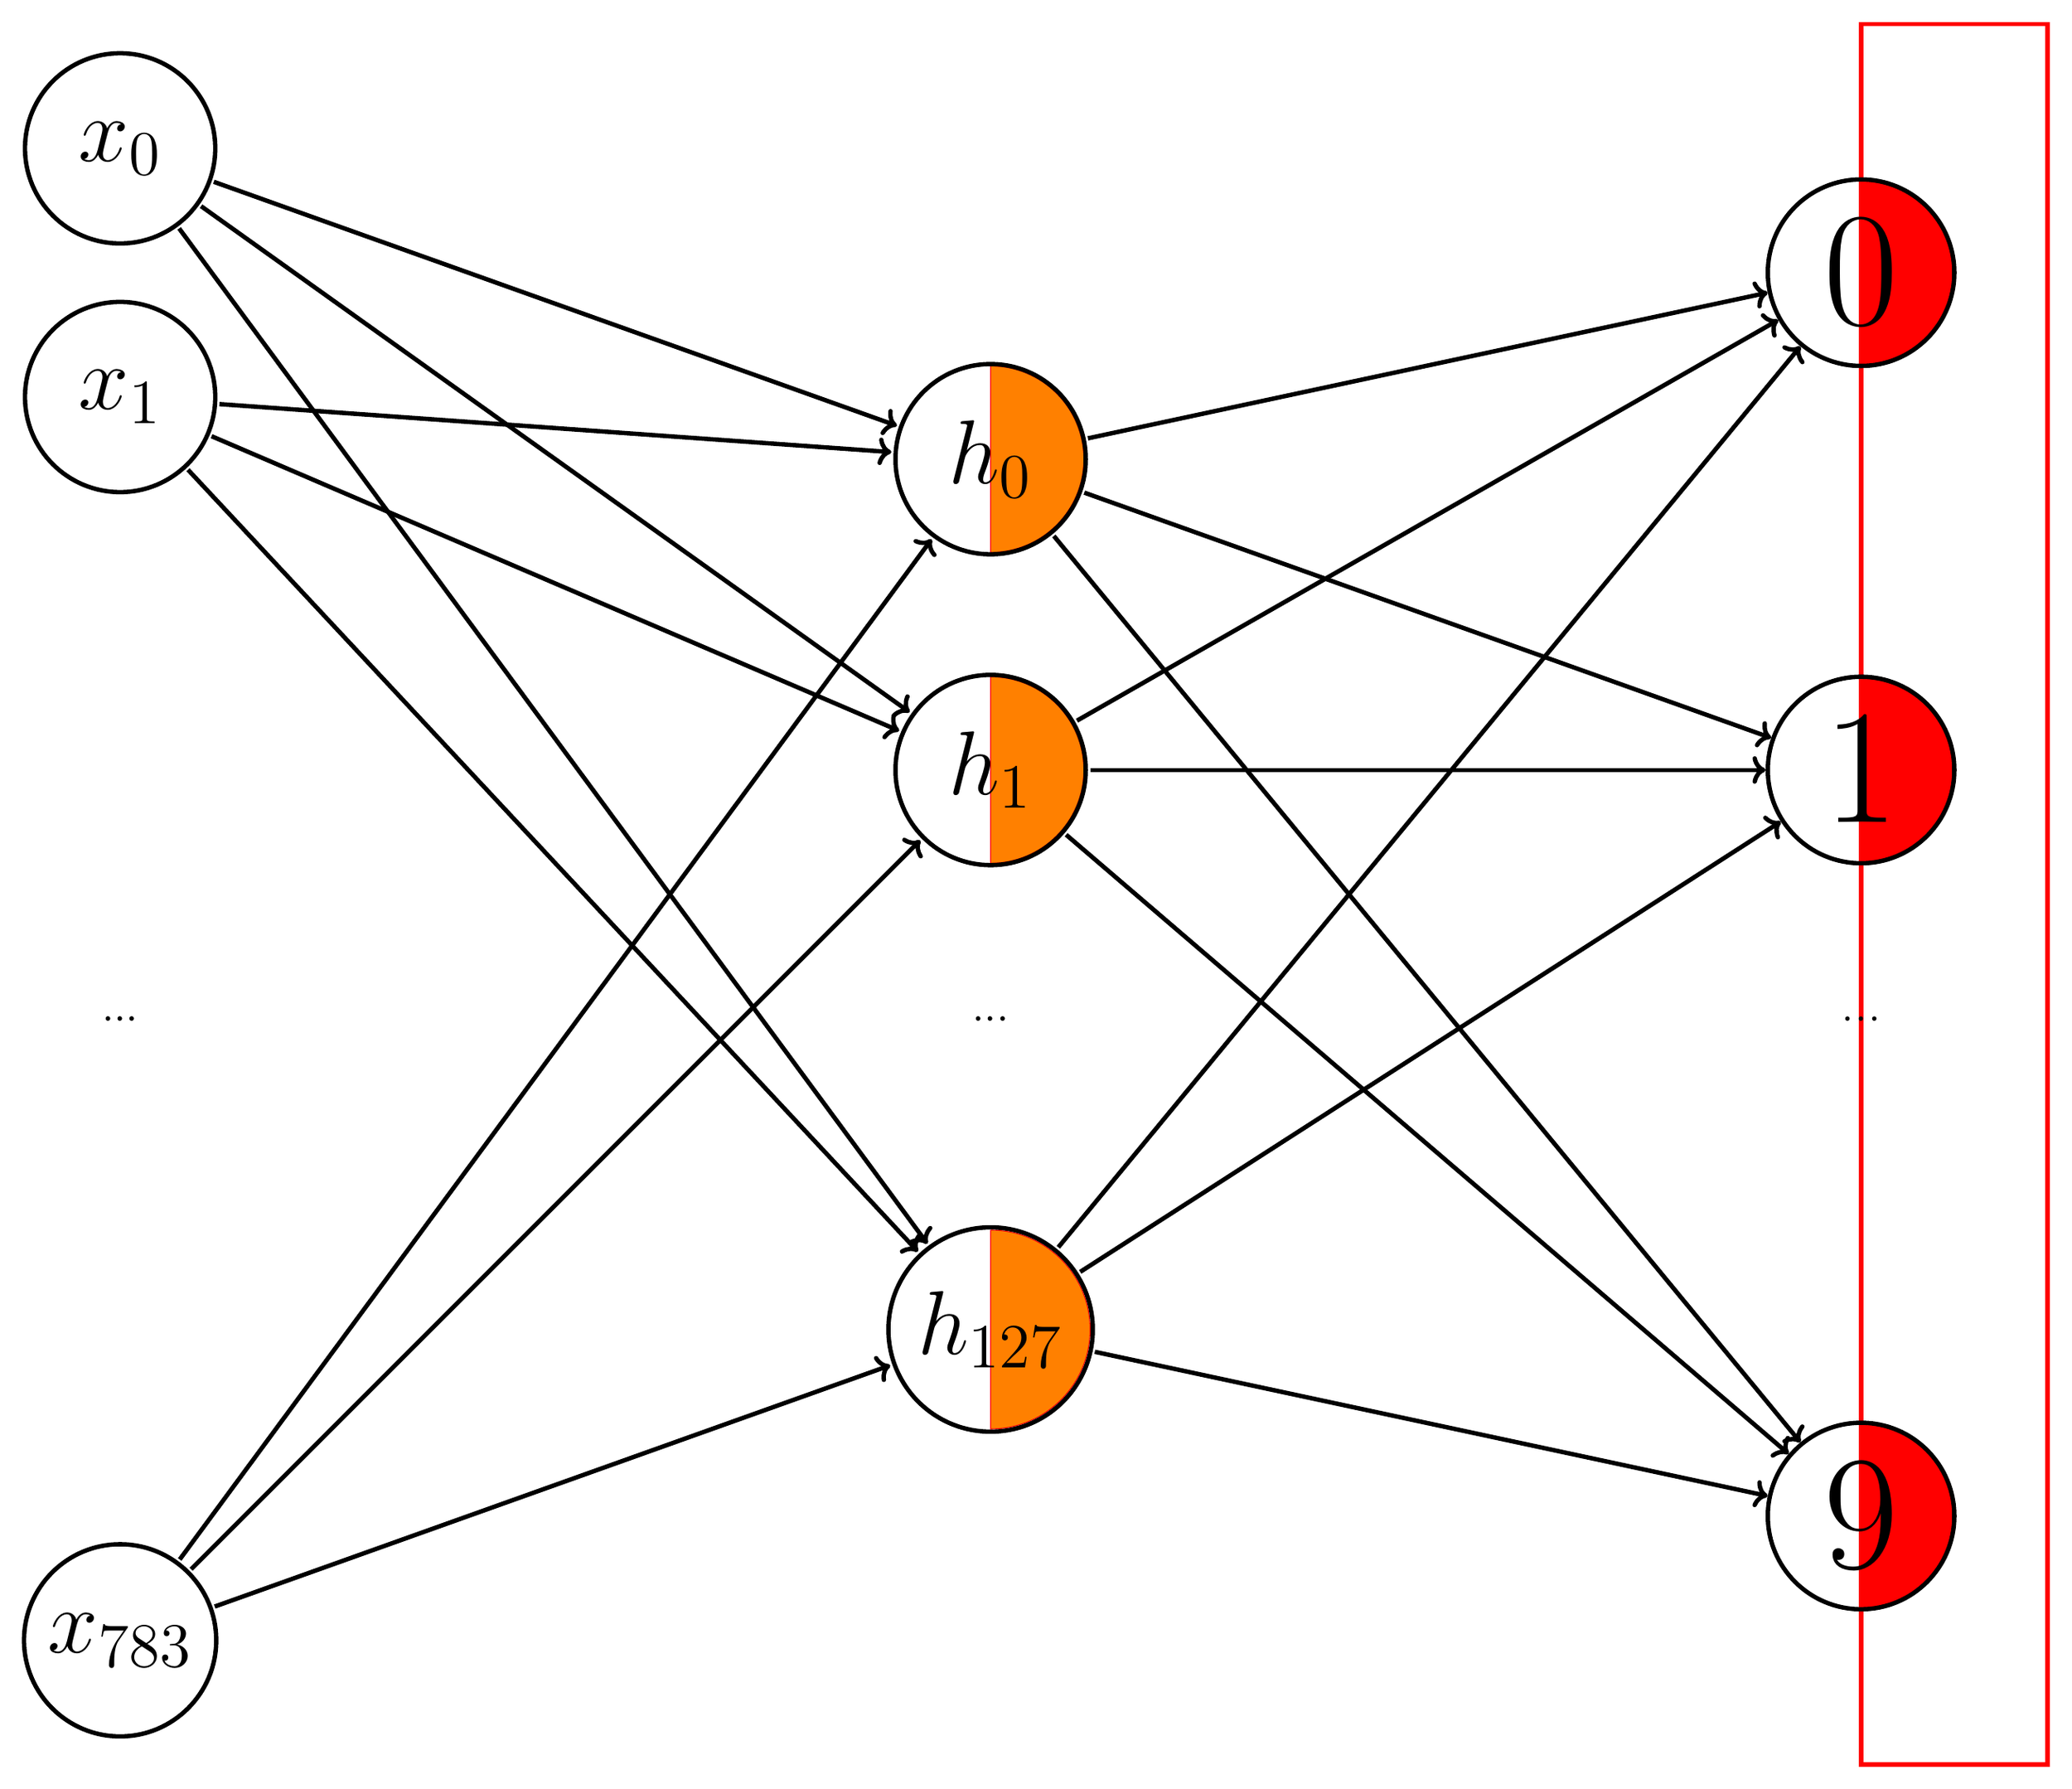
\begin{tikzpicture}

% modify thickness

% input nodes

\node[draw, scale=2, line width=2, circle, minimum size=1.53cm] (x0) at (-7, 12) {\huge $x_0$};
\node[draw, scale=2, line width=2, circle, minimum size=1.53cm] (x1) at (-7, 8) {\huge $x_1$};
\node[scale=2, line width=2, circle, minimum size=1.53cm] (xother) at (-7, -2) {$...$};
\node[draw, scale=2, line width=2, circle, minimum size=1cm] (x783) at (-7, -12) {\huge $x_{783}$};

% right hemisphere of hidden nodes
\draw[red, fill=orange] (7,8.5) arc(90:-90:1.5) -- (7,6.5) -- (7,8.5);
\draw[red, fill=orange] (7,3.5) arc(90:-90:1.5) -- (7,1.5) -- (7,3.5);
\draw[red, fill=orange] (7,-5.4) arc(90:-90:1.6) -- (7,-7.4) -- (7,-5.4);

% right hemisphere of hidden nodes
%\draw[red, fill=red] (7,8.5) arc(90:-90:1.5) -- (7,6.5) -- (7,8.5);
%\draw[red, fill=red] (7,3.5) arc(90:-90:1.5) -- (7,1.5) -- (7,3.5);
%\draw[red, fill=red] (7,-5.4) arc(90:-90:1.6) -- (7,-7.4) -- (7,-5.4);

% rectangle around x
\draw[line width=2, color=red] (21, 14) rectangle (24, -14);

% hidden nodes

\node[draw, scale=2, line width=2, circle, minimum size=1.53cm] (h0) at (7, 7) {\huge $h_0$};
\node[draw, scale=2, line width=2, circle, minimum size=1.53cm] (h1) at (7, 2) {\huge $h_1$};
\node[scale=2, line width=2, circle, minimum size=1.53cm] (hother) at (7, -2) {$...$};
\node[draw, scale=2, line width=2, circle, minimum size=1cm] (h127) at (7, -7) {\huge $h_{127}$};


% right hemisphere of output nodes
\draw[red, fill=red] (21,11.5) arc(90:-90:1.5) -- (21,9.5) -- (21,11.5);
\draw[red, fill=red] (21,3.5) arc(90:-90:1.5) -- (21,1.5) -- (21,3.5);
\draw[red, fill=red] (21,-8.5) arc(90:-90:1.5) -- (21,-10.5) -- (21,-8.5);

% output nodes

\node[draw, line width=2, circle, minimum size=3cm] (y0) at (21, 10) {};
\node[draw, line width=2, circle, minimum size=3cm] (y1) at (21, 2) {};
\node[line width=2, minimum size=3cm] (yother) at (21, -2) {\Huge ...};
\node[draw, line width=2, circle, minimum size=3cm] (y9) at (21, -10) {};

\node[scale=3] (y0_label) at (21,10) {\Huge 0};
\node[scale=3] (y1_label) at (21,2) {\Huge 1};
\node[scale=3] (y9_label) at (21,-10) {\Huge 9};


% input to hidden
\draw [->, line width=2] (x0) -- (h0); 
\draw [->, line width=2] (x0) -- (h1); 
\draw [->, line width=2] (x0) -- (h127);

\draw [->, line width=2] (x1) -- (h0); 
\draw [->, line width=2] (x1) -- (h1); 
\draw [->, line width=2] (x1) -- (h127); 

\draw [->, line width=2] (x783) -- (h0); 
\draw [->, line width=2] (x783) -- (h1); 
\draw [->, line width=2] (x783) -- (h127); 


% hidden to output
\draw [->, line width=2] (h0) -- (y0); 
\draw [->, line width=2] (h0) -- (y1); 
\draw [->, line width=2] (h0) -- (y9);

\draw [->, line width=2] (h1) -- (y0); 
\draw [->, line width=2] (h1) -- (y1); 
\draw [->, line width=2] (h1) -- (y9); 

\draw [->, line width=2] (h127) -- (y0); 
\draw [->, line width=2] (h127) -- (y1); 
\draw [->, line width=2] (h127) -- (y9); 



\end{tikzpicture}
\end{document}